\documentclass[openany]{book}
\usepackage[utf8]{inputenc}
\usepackage{verbatim}
%%%%%%%%%%%%%%%%%%%%%%%

%%%%%%%%%%%%%%%%%%%%%%%
% HOLA PACO
% ESTE ES EL ARCHIVO DE LAS DEFINICIONES ESTRUCTURALES
% VERSION 1.1 NOMÁS
%
% AUTOR ORIGINAL:
% EDUARDO (CHITO) BELMONTE GUILLAMÓN
%
% ESTE ARCHIVO ES COMUNISTA, PUEDES COMPARTIRLO SI QUIERES
%%%%%%%%%%%%%%%%%%%%%%%

%----------------------------------
%     PAQUETICOS QUE SE USAN
%----------------------------------

%--------------------------
%    PARA USAR INKSCAPE
%---------------------------
\usepackage{import}
\usepackage{hyperref}
\usepackage{xifthen}
\usepackage{pdfpages}
\usepackage{transparent}

\newcommand{\incfig}[1]{%
    \def\svgwidth{\columnwidth}
    \import{./figures/}{#1.pdf_tex}
}

\newcommand{\custincfig}[2]{%
    \def\svgwidth{#1}
    \import{./figures/}{#2.pdf_tex}
}
\newcommand{\textnexttofig}[3]{
  \begin{minipage}[l]{0.45\textwidth}
    \custincfig{#1}{#2}
  \end{minipage}
  \begin{minipage}[l]{0.45\textwidth}
    #3
  \end{minipage}
}

%%%%%%%%% FIN DEL INKSCAPE

\usepackage{parskip} % Pa parrafos wapos
\setlength{\parindent}{0.5cm} % Pa la sangría
\usepackage{graphicx} % Pa meter las imágenes
\graphicspath{{Images/}} % La ruta a las imágenes

\usepackage{tikz} % Pa dibujar cosichuelas guapas

\usepackage[spanish]{babel} % PA QUE ESTÉ EN ESPAÑOL NOMÁS

\usepackage{enumitem} % Para personalizar las LISTAS YEAH

\setlist{nolistsep} % Pa que las listas estén junticas

\usepackage{booktabs} % Esta sirve para hacer tablas fancy con multicolumns y tal pero no tengo ni puta idea de usarla

\usepackage{xcolor} % PA DEFINIR LOS COLORINES
\definecolor{turquoise}{RGB}{21,103,112} % Es un turquesica así formal
\definecolor{violet}{RGB}{ 110, 6, 187 } % Color maricón

%-------------------------------------------------
%     MÁRGENES
%-------------------------------------------------

\usepackage{geometry}
\geometry{
    top=3cm,
    bottom=3cm,
    left=3cm,
    right=3cm,
    headheight=14pt,
	footskip=1.4cm,
	headsep=10pt,
}

\usepackage{avant} % Esto es una fuente para encabezados

%\usepackage{mathptmx} % Usar simbolitos matemáticos chulos

\usepackage{microtype} % Para fuentes de maricones

\usepackage[utf8]{inputenc} % Pa los acentos

\usepackage[T1]{fontenc}

%-------------------------------------------------
% Bibliografía e índice
%-------------------------------------------------

\usepackage{makeidx} % Pa hacer un índice
\makeindex

\usepackage{titletoc}   % Para manipular la tabla de contenidos

\contentsmargin{0cm}    % Para eliminar el margen por defecto

\usepackage{titlesec} % Pa cambiar los titulos skere

\titleformat
{\chapter} % command
[display] % shape
{\centering\bfseries\Huge\normalfont} % format
{\color{turquoise}  {\normalsize\MakeUppercase{Capítulo} \thechapter }} % label
{-0.5cm} % sep
{
    \color{turquoise}
    \rule{\textwidth}{3pt}
    \vspace{1ex}
    \centering
    \setcounter{ex}{0}
    \setcounter{dummy}{0}
} % before-code
[
\vspace{-0.5cm}%
\rule{\textwidth}{3pt}
] % after-code


\titleformat{\part}
[display]
{\centering\bfseries\Huge\normalfont}
{\color{turquoise} {\normalsize \MakeUppercase{Asignatura}}}
{0pt}
{\color{turquoise}
\vspace{-0.6cm}
\rule{\textwidth}{3pt}
\vspace{1ex}
\setcounter{chapter}{0}
\setcounter{section}{0}
\setcounter{dummy}{0}
\centering
}


\titleformat{\section}
{\normalfont\Large\bfseries}{\color{turquoise}\thesection\ - }{0.5em}{}

\usepackage{fancyhdr}   % Necesario para el encabezado y el pie de página

\pagestyle{fancy}   %Para modificar los encabezados
\fancyhf{}          %Para eliminar los encabezados y pies de página por defecto.
\fancyhead[LE,RO]{\sffamily\normalsize\thepage}
\fancyfoot[C]{Ampliación de Probabilidad}
%HACER

\usepackage{amsmath,amsfonts,amssymb,amsthm,cancel} % PARA LAS MATES

%   LINEA 199, HACER CAPULLADAS

\newtheoremstyle{turquoisebox}
{0pt} %Espacio encima
{0pt} %Espacio abajo
{\normalfont} % Fuente del cuerpo
{} % Cantidad de identado
{\small\ssfamily\color{turquoise}} % Fuente en la que pone "TEOREMA"
{:} % Puntuación tras el teorema
{0.25em} %Espacio tras el teorema
{\thmname{#1}\thmnumber{#2}} %No sé si esto funciona


\newcounter{dummy}
\newcounter{ex}
\newtheorem{teoremote}[dummy]{\color{turquoise}Teorema}
\newtheorem{propositiont}{\color{turquoise}Proposición}[section]
\newtheorem{lemmat}{\color{turquoise}Lema}[section]
\newtheorem{definitionT}{\color{turquoise}Definición}[section]
\newtheorem{exerciseT}[ex]{Ejercicio}
\newtheorem{examplote}[ex]{\color{turquoise}Ejemplo}
\newtheorem{methodT}[dummy]{\color{turquoise}Método}


\RequirePackage[framemethod=default]{mdframed} % Required for creating the theorem, definition, exercise and corollary boxes

%Caja de teoremas

\newmdenv[skipabove=7pt,
skipbelow=7pt,
backgroundcolor=black!5,
linecolor=turquoise,
innerleftmargin=5pt,
innerrightmargin=5pt,
innertopmargin=5pt,
leftmargin=0cm,
rightmargin=0cm,
linewidth=3pt,
innerbottommargin=5pt]{tBox}

\newmdenv[skipabove=7pt,
skipbelow=7pt,
backgroundcolor=black!5,
linecolor=turquoise,
innerleftmargin=5pt,
innerrightmargin=5pt,
innertopmargin=5pt,
leftmargin=0cm,
rightmargin=0cm,
linewidth=1pt,
innerbottommargin=5pt]{pBox}

\newmdenv[skipabove=7pt,
skipbelow=7pt,
backgroundcolor=violet!7,
linecolor=turquoise,
innerleftmargin=5pt,
innerrightmargin=5pt,
innertopmargin=5pt,
leftmargin=0cm,
rightmargin=0cm,
rightline=false,
topline=false,
bottomline=false,
linewidth=4pt,
innerbottommargin=5pt]{mBox}

\newmdenv[skipabove=7pt,
skipbelow=7pt,
rightline=false,
leftline=true,
topline=false,
bottomline=false,
linecolor=turquoise,
innerleftmargin=5pt,
innerrightmargin=5pt,
innertopmargin=0pt,
leftmargin=0cm,
rightmargin=0cm,
linewidth=4pt,
innerbottommargin=0pt]{dBox}

\newmdenv[skipabove=7pt,
skipbelow=7pt,
rightline=false,
leftline=true,
topline=false,
bottomline=false,
backgroundcolor=black!3,
linecolor=turquoise!50,
innerleftmargin=5pt,
innerrightmargin=5pt,
innertopmargin=0pt,
innerbottommargin=5pt,
leftmargin=0cm,
rightmargin=0cm,
linewidth=4pt]{eBox}

\newmdenv[skipabove=7pt,
skipbelow=7pt,
leftline=true,
topline=false,
rightline=false,
bottomline=false,
backgroundcolor=cyan!5,
linecolor=turquoise,
innerleftmargin=5pt,
innerrightmargin=5pt,
innertopmargin=0pt,
innerbottommargin=5pt,
leftmargin=0cm,
rightmargin=0cm,
linewidth=4pt]{exBox}

\newenvironment{theorem}{\begin{tBox}\begin{teoremote}}{\end{teoremote}\end{tBox}}
\newenvironment{proposition}{\begin{pBox}\begin{propositiont}}{\end{propositiont}\end{pBox}}
\newenvironment{lemma}{\begin{pBox}\begin{lemmat}}{\end{lemmat}\end{pBox}}
\newenvironment{method}{\begin{mBox}\begin{methodT}}{\end{methodT}\end{mBox}}
\newenvironment{definition}{\begin{dBox}\begin{definitionT}}{\end{definitionT}\end{dBox}}
\newenvironment{exercise}{\begin{eBox}\begin{exerciseT}}{\hfill{\color{black}}\end{exerciseT}\end{eBox}}
\newenvironment{example}{\begin{exBox}\begin{examplote}}{\end{examplote}\end{exBox}}
\newenvironment{demonstration}{\begin{flushright}
      \color{turquoise} \textbf{Demostración}
\end{flushright}
}{\begin{flushright}
  $\square$
\end{flushright}}

\usepackage{geometry}
\geometry{
    top=3cm,
    bottom=3cm,
    left=3cm,
    right=3cm,
    headheight=14pt,
	footskip=1.4cm,
	headsep=10pt,
}
\usepackage{graphicx}
\title{Ecuaciones en Derivadas Parciales y Series de Fourier}
\author{Colaboración estelar entre Paco Mora 
\includegraphics[scale=0.02]{cosmo} y Chito Belmonte 
\includegraphics[scale=0.13]{wanda}}
\date{\today}

\begin{document}
\maketitle

\tableofcontents

\textbf{En el caso de detección de errores o erratas, agradecemos el contacto a la dirección \textit{eduardo.belmonteg@um.es}}

\chapter{Qué chuchas es una ecuación en derivadas parciales} %barras

\subsection{Introducción a EDP}
\begin{minipage}[l]{0.6\textwidth}
  Hemos visto teoría sobre \textit{Ecuaciones Diferenciales Ordinarias}. Su característica de \textit{Ordinaria} es que sólo se deriva con respecto a una variable.
\end{minipage}
\begin{minipage}[l]{0.4\textwidth}
  $$ x'(t)=f(t) \to x(t) = \int f + K $$
\end{minipage}

La familia de soluciones en este caso depende de un parámetro real. Otros tipos de EDO's tienen otro métodos de resolución, como ya vimos.

\begin{minipage}[l]{0.5\textwidth}
  Por contra, las ecuaciones en derivadas parciales tienen un aspecto distinto.
\end{minipage}
\begin{minipage}[l]{0.5\textwidth}
  $$ \dfrac{\partial u}{\partial x}(x,y)=f(x,y) \to \int f(x,y)dx +g(y) $$
\end{minipage}

La familia de soluciones depende en este caso de un parámetro que es una función.

La teoría de \textit{Ecuaciones en Derivadas Parciales} consiste en el estudio de algunas funciones, que cumplen determinadas condiciones que nos facilitan su estudio. En muchas ocasiones, nos encontraremos con casos en los que no podamos determinar nada sobre la solución.

La teoría para ecuaciones en derivadas parciales de primer orden es bastante sencilla. Se reduce a un sistema de lineas a partir de las cuales se puede construir la superficie solución de la ecuación. Este caso de estudio es poco útil, por eso casi siempre nos encontraremos ecuaciones de orden dos o superior.

\begin{minipage}[l]{0.1\textwidth}
  
\includegraphics[scale=0.2]{wanda}
\end{minipage}
\begin{minipage}[l]{0.8\textwidth}
  No vamos a representar en este texto la bonita charla que está dando Matías sobre la primera EDO de la historia y su relación con Sir Isaac Newton, Francisco Misco y el holocausto judío pero es bastante interesante.
\end{minipage}

\subsection{Ejemplos de EDPs}
\subsubsection{Ecuación de ondas}
\begin{minipage}[l]{0.1\textwidth}
  
\includegraphics[scale=0.2]{wanda}
\end{minipage}
\begin{minipage}[l]{0.8\textwidth}
  Nos está dando una bonita charla sobre muchas ecuaciones y todavía no ha hablado de ondas... Ya han pasado 25 minutos, auxilio.
\end{minipage}


Esta modelando como se deforma una cuerda en un punto cuando se le aplica una pequeña fuerza para ello coje un incremento en el eje $x$, ($\Delta x$) y calcula el angulo en el punto $x$ y en $x + \Delta x$, y esto lo pone en funcion de la curva $U(x,t)$:
$$tg(\alpha) = \dfrac{\partial u}{\partial x} (x + \Delta x, t) \hspace{1cm} tg(\beta) = \dfrac{\partial u}{\partial x}(x,t)$$

Como trabajar con tangentes es muy complicado aproximamos la tangente mediante el angulo: $tg(\alpha) \sim \alpha$.
Ahora simplemente restamos estos dos ángulos y multiplicamos por la tensión (T), y esto debe ser una fuerza que como sabemos es masa por aceleración. La masa viene dada por $\rho \Delta x$
donde $\rho$ es la densidad de masa por longitud (constante). La aceleracion es la derivada segunda de $U(x,t)$ respecto de $t$ quedando por tanto la siguiente ecuacion:
$$ T\left(\dfrac{\partial u}{\partial x} (x + \Delta x, t) - \dfrac{\partial u}{\partial x}(x,t) \right) = F =  \rho \Delta x \dfrac{\partial ^2 u}{\partial t ^2}(x,t)  $$
$$ T\left(\dfrac{\dfrac{\partial u}{\partial x} (x + \Delta x, t) - \dfrac{\partial u}{\partial x}(x,t)}{\partial x}\right) = \rho \dfrac{\partial ^2 u}{\partial t^2} (x,t)$$
Tomando el limite $ \Delta x \to 0 $
$$ T \dfrac{\partial ^2 u}{\partial x ^2}(x,t) = \rho \dfrac{\partial ^2 u}{\partial t ^2}(x,t)   $$

Llegamos a la ecuación de ondas:
$$ \dfrac{\partial ^2 u}{\partial x ^2}- \dfrac{\rho}{T} \dfrac{\partial ^2 u}{\partial t ^2} = 0 $$
Cuya solución podemos calcular haciendo $ \rho/T = 1/c ^2 $, la ecuación queda $ \dfrac{\partial ^2 u}{\partial x ^2}-  \dfrac{1}{c ^2} \dfrac{\partial ^2 u}{\partial t ^2} = 0 $, entonces algunas soluciones son:

$$ u(x,t) = f(x+ct)\hspace{1cm}\dfrac{\partial ^2 u}{\partial x ^2} = f''(x+ct)\hspace{1cm} \dfrac{\partial ^2 u}{\partial t} = c ^2 f''(x+ct)  $$

$$ u(x,t) = f(x+ct)-g(x-ct) $$
% vaya puto porro chat asies
%okey sisi
% Ahora si que estoy un poco perdido espero que os esteis enterando
Sabemos que $ u(0,t)=u(2,t)=0 $ y entonces:

$$ f(ct) +g(-ct) = 0 \forall t \implies f(x) = -g(-x) \ \forall x$$
$$ f(1+ct) +g(1-ct) = 0 \forall t \implies f(x+2)=-g(-x)\ \forall x $$
Por tanto, $ f(x) = f(x+2) $ y $ f $ es 2-periódica.


Coje un muelle le pone una masa gorda al final, desde esa masa saca otro muelle hacia delante y le pone otra masa y asi continuamente, y llama al desplazamiento de la masa $n$  $U(n,t)$ donde la $n$ es un numero natural que indica cual de las masas estamos cogiendo y la $t$ es como siempre el tiempo. Ahora cogemos y restamos una masa con la anterior para aplicar la ley de hook a un solo muelle entre dos masas ''contiguas'', $F=K \cdot x$, de forma que se nos queda la siguiente ecuacion:

%voy copiando lo que pone, explicalo tu
% va lo intento xd

$$ k(U(n-1,t)-U(n,t))-k(U(n,t).U(n+1,t)) = m \dfrac{\partial ^2 u}{\partial t ^2}(n,t)  $$
donde la $k$ es la constante del muelle, $m$ es la masa y $\dfrac{\partial ^2 u}{\partial t ^2}(n,t)$ es la aceleracion.
$$ U(n+1,t)-2U(n,t)+U(n-1,t) = m \dfrac{\partial ^2 u}{\partial t ^2}(n,t) $$
Tomando límites, el primer miembro nos recuerda a la segunda derivada:
$$ \lim_{h \to 0} \dfrac{f(x+h)-2f(x)+f(x-h)}{h ^2} = \dfrac{f'(x+h)-f'(x-h)}{2h}=f''(x)   $$

Volviendo a nuestra ecuación:
$$ k \dfrac{\partial ^2(x,t)}{\partial x ^2} (\Delta x)^2 = \rho \Delta x \dfrac{\partial ^2 (x,t)}{\partial t ^2}  $$
La constante del muelle ($k$) depende de la longitud del muelle por tanto le afecta el incremento de x $(\Delta x)$:
$$ \dfrac{k}{\cancel{\Delta x}}  \dfrac{\partial ^2u(x,t)}{\partial x ^2} \cancel{(\Delta x)^2} = \rho \cancel{\Delta x} \dfrac{\partial ^2 u(x,t)}{\partial t ^2}  $$

Con lo que nos queda la ecuación de ondas que vimos anteriormente.

% Ahora hablemos de terremotos donde aplicaremos estas ecuaciones que hemos obtenidos. Dibuja la tierra y ondas en la superficie que se acercan cada vez mas al centro de ella.
% IMPOSIBLE DE COPIAR O ENtender ESto
%chavales se comenta, no se borra nada por si no deja hacer control z
%OUCH

%%%%%%vale es un caso concreto yo sudaria

% Estas no son horas de llamar a menos que me la quieras mamar que quieras joder que quieras chingar

%Mucha diferencia de presión pero a mi EDP me está dando depresión
%barras, de verdad esto que es;⪺€çÏâöඞ
%Alguien sabe lo que es la V si el volumen aaa
% Esoera no copies mucho que el payo no sabe por donde empezar
%introduzco solo

Para ilustrar la ecuación de ondas que acabamos de estudiar creamos un modelo de un recipiente en el que se puede desplazar una barra. La P es la presión y V es el volumen del recipiente.

\begin{center}
  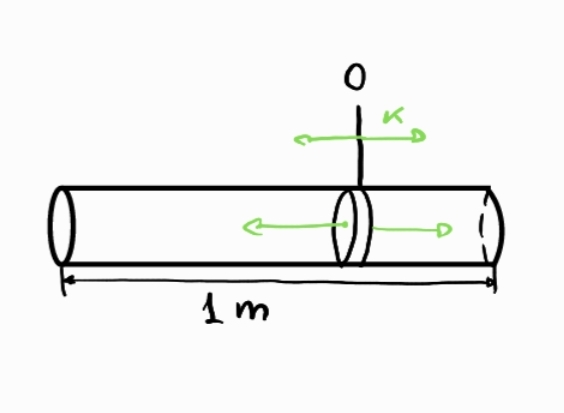
\includegraphics[scale=0.3]{EDP1.jpg}
\end{center}
$$ \cancel{P} = (P-\Delta P)(1+x)= \cancel{P} - \Delta P +xP -\underbrace{\Delta P}_{\sim 0} $$
$$ \Delta P = -xP $$
%creo que acaba de decir que va a hacer apuntes decentes
% Yo si fuera tú sudaría. idk por si acaso, si no comentamos todo
%no esta haciendo nada no?
%nop

\begin{minipage}[l]{0.1\textwidth}
 
\includegraphics[scale=0.02]{cosmo}
 \end{minipage}
 \begin{minipage}[l]{0.8\textwidth}
 Seguimos con las introducciones físicas que no sabemos de dónde vienen ni a dónde van.
 \end{minipage}


%no se que hace, yo copio:
Tenemos un cilindro con un fluido, queremos calcular la presión en función de la altura de un fluido contenido en un cilindro vertical. Para ello calculamos las fuerzas que se ejercen.
La primera es la generada por la presión atmosférica que se encuentra en el eje vertical, la segunda es (no se cual es la que va hacia arriba tiene que ser otra presión) y luego el peso del fluido. La suma de estas fuerzas tiene que ser 0 pues el fluido esta en reposo por tanto tenemos que la diferencia de presión entre dos puntos($z$ y $\Delta z$) multiplicada por la superficie del agua superficial (que nos da una fuerza), y el peso es $g\rho \Delta x$ donde $g$ es la gravedad y $\rho$ la densidad han de ser iguales.
%figura del Karbajo
 $$ p\omega = g \rho S \Delta z $$
 $$ (P(z)-P(z+\Delta z))\cancel S = g \rho \cancel{S} \Delta z $$
 Si pasamos el $\Delta x$ dividiendo y hacemos el limite obtenemos:
 $$ \dfrac{\partial p}{\partial x} = \dfrac{\partial p}{\partial y}=0  \hspace{1cm} \dfrac{\partial p}{\partial z} = \rho g $$
$$ \triangledown p = (0,0,-\rho g) $$

Vamos a resolver la ecuacion:
$$ \rho \sim cp $$
$$ - \dfrac{\partial p}{\partial z} = cp(z) $$
$$ -p'(z)=cp(z) \hspace{1cm} \dfrac{p'}{p} = -c \hspace{1cm} p(z) = p_0 \rho ^{-cz} $$
$  $\\

\textbf{Ecuación de los fluidos}\\
%dibujo del Karbajo
Tenemos una corriente en un fluido no compresible y nos fijamos en una seccion (S) orientada (tenemos un vector normal) y queremos medir que cantidad de fluido atraviesa S. Tenemos que la velocidad del fluido (v) depende de la posicion (x,y,z) y del tiempo. Y para modelar la masa que atraviesa la seccion (masa saliente de la seccion) por unidad de tiempo hacemos este calculo:
$$ \underbrace{\rho \overrightarrow{S} \overrightarrow{v}\Delta t }_{\text{masa saliente}} \to \underbrace{\iint_{\partial D} \rho \overrightarrow{v}d \overrightarrow{S}}_{\text{integral de flujo}} $$

Podemos aplicar el teorema de Gauss-Ostrogadsky para convertir esta integral en una integral triple.

$$ \iint_{\partial D}\rho \overrightarrow{v}d \overrightarrow{S} = \iiint_D \rho dV  $$

\subsection{Ecuación de calor.Procesos de difusión}

Tomemos una región confinada de moléculas que se mueven de manera caótica, cada partícula tiene una trayectoria propia. Seguimos de forma estadística las trayectorias.

Sean $ X,Y $ una variables aleatorias. Cuando son independientes sus funciones de densidad $ f(x),g(y) $ cumplen que $ f(x)\cdot g(y) $ el densidad conjunta.
Como consecuencia, si tenemos un conjunto
$$P((X,Y \in A)) = \iint_A f(x,y) dxdy $$

Para calcular la función de distribución de $ X+Y $ (es decir, $P(X+Y \leq Z$) se procede de este modo:

$$ P (X+Y \leq z) = \iint_{x+y \leq  z} f(x)g(y)dxdy $$

Para calcular esta integral podemos hacer el cambio de variable $ x=s,\ x+y=z $, de forma que la integral queda:

$$ = \int_{-\infty}^{z}\underbrace{ \left(\int_{-\infty}^{+\infty}f(s)g(z-s)ds \right) }_{ \text{densidad de }X+Y\text{, la convolución} } dz $$

% se está fumando un porro

Cuando apliquemos esto a una función $ f(x,t) $ que represente una eucación diferencial, usando una v.a. densidad $\phi$ con varianza proporcional al incremento del tiempo obtenemos lo siguiente:

$$ f(x,t+\tau) = \int_{-\infty}^{+\infty} = f(x+\xi,t)\phi(\xi)d\xi = \int_{-\infty}^{+\infty}\left(f(x,t)+ \dfrac{\partial f}{\partial x}(x,t)\xi + \dfrac{1}{2} \dfrac{\partial ^2 f}{\partial x ^2} (x,t) \xi\right) \phi(\xi) d\xi $$
$$\simeq f(x,t)+ \dfrac{\partial ^2 f}{\partial x ^2}(x,t)c\tau \implies \dfrac{\partial f}{\partial t} = c \dfrac{\partial ^2f }{\partial x ^2} $$

\begin{minipage}[l]{0.1\textwidth}
    
\includegraphics[scale=0.2]{wanda}
\end{minipage}
\begin{minipage}[l]{0.8\textwidth}
  Ahora olvidaos de toda la \textbf{bullshit} que hemos visto que comienza el espectáculo, empieza el temario.
\end{minipage}

\section{Qué es una EDP}

\begin{definition}
  { \color{turquoise} \textbf{Ecuación en Derivadas Parciales}}

  Una \textbf{EDP} es una ecuación de la forma

  $$ F\left(x_1, x_2, x_3,..., \dfrac{ \partial u}{\partial x_1},\dfrac{ \partial u}{\partial x_2}, ..., \dfrac{ \partial^n u}{??} \right) $$

  Con $ u $ una función doblemente derivable.
\end{definition}

Su diferencia fundamental con las $ EDOs $ es... ª

La expresión general de una EDP es $$ f(x,u)=u' $$

Si se le añade una condición inicial, estamos ante un problema de Cauchy, pero tal cual está expresado sus soluciones no son únicas. Aquí aparecen lo que se llaman 'soluciones singulares'.

\begin{definition}
  { \color{turquoise} \textbf{EDP de Primer Orden}}

  $$ F \left( x_1, x_2, ... , \dfrac{\partial u}{\partial x_1},\dfrac{\partial u}{\partial x_2},...,u  \right)=0 $$
\end{definition}

Dice Matías que no le gusta esta ecuación así que en su lugar nos va a explicar otra

\begin{definition}
  { \color{turquoise} \textbf{Ecuación quasi-lineal en dos variables}}

  $$ A(x,y,u) \dfrac{\partial u}{\partial x}+B(x,y,u)\dfrac{\partial u}{\partial y}=C(x,y,u) $$
\end{definition}

Estas son las primeras que vamos a resolver y, a partir de estas, veremos las soluciones de una EDP de primer orden. Para una EDP de segundo orden, pueden aparecer derivadas mixtas (cosa que no aparece en los ejemplos), y la teoría nos dice que con los cambios oportunos de variable se pueden hacer desaparecer las derivadas mixtas de problemas de cierta generalidad, y hacerlos semejante a las soluciones de una EDP de primer orden con la que ya estamos familiarizados.

\vspace{1cm}

\begin{minipage}[l]{0.1\textwidth}
    
\includegraphics[scale=0.2]{wanda}
\end{minipage}
\begin{minipage}[l]{0.8\textwidth}
  Han sido unos maravillosos 24 minutos de lucidez de Matías. Ahora ha vuelto a hablar de curvas y dibujitos y está sufriendo una embolia en la pizarra. Aprovecho para contaros un chiste: Un matemático, un físico y un biólogo están mirando una casa. En la casa entran dos personas y salen tres. El físico dice 'Ha debido de ser un error en la medición'. El biólogo dice 'No, es probable que se hayan reproducido'. El matemático dice 'Si entra una persona más, la casa se queda vacía'.
\end{minipage}

\vspace{1cm}

\begin{definition}
  Llamamos ecuaciones cuasi-lineales a las que son de la forma:

  $$ A \dfrac{\partial u}{\partial x} + B \dfrac{\partial u}{\partial y} = C $$

  Donde $ A,B,C: \Omega \subset \mathbb{R}^3 \to \mathbb{R}\ C ^{1} $ ($ A,B,C $ son de la forma $ A(x,y,u) $ y $ u $ es de la forma $ u(x,y) $)

\end{definition}



% Vamos a considerar el siguiente sistema
%
% $$ \left\{ \begin{array}{l}
%   x'=A(x,y,z)\\
%   y'=B(x,y,z)\\
%   z'=C(x,y,z)\\
%   (x(0), y(0), z(0)) = p
% \end{array} \right. $$
%
% PACO AQUÍ NO SÉ LO QUE HA PASADO, SE HA FUMADO CUATRO PORROS

\begin{theorem}
    Consideremos el sistema autónomo de Cauchy:
    $$
    \left\{
    \begin{array}{l}
        x'=A(x,y,z)\\
        y'=B(x,y,z)\\
        z' = C(x,y,z)\\
        (x(0),y(0),z(0))=P

    \end{array}
    \right.
    $$
    definido en $ S = \{ (x,y,z)\ :\ z = u(x,y) \} $
    Entonces si $ p \in S $, toda la órbita solución $ (x(t),y(t),z(t)) \in S $ donde $ u  $ es solución del sistema.
\end{theorem}

% El porro aqui:
% Obtenemos una curva solución del sistema $(x(t), y(t), z(t))$ que pasa por $P$ en $t=0$. Tomamos una curva alternativa $(x(t), y(t), u(x(t)), y(t))$, que en $t=0$ también pasa por $P$. Comprobaremos que  la curva alternativa es solución coordenada a coordenada.
%
% $$ A(x(t),y(t),z(t))=x'(t) =? A(x(t),y(t),u(x(t),y(t))) $$
%
% $$ \dfrac{d}{dt} (u(x(t)),y(t)) = \dfrac{\partial u}{\partial x}(x(t), y(t))\underbrace{ x'(t) }_{ A(x,y,z) } + \dfrac{\partial u}{\partial y}(x(t), y(t))y'(t)$$

Dada la ecuación:
  $$     \left\{
      \begin{array}{l}
          x'=A(x,y,z)\\
          y'=B(x,y,z)\\
          z' = C(x,y,z)\\
          (x(0),y(0),z(0))=P

      \end{array}
      \right. $$

Dada $ \Gamma(t,s) $ a la solución de la ecuación y que pasa por $ \gamma(s) $, es decir, $ \Gamma(0,s) = \gamma(s) $, al ser $ \Gamma $ solución sabemos también que:
$$ \dfrac{\partial \Gamma}{\partial t} (t,s) = A(\Gamma(t,s)) \forall s,\forall t \footnote{que estén dentro de un cierto entorno}$$



%%lo que hay hasta ahora de lectures (9/2)

% Tomemos la ecuación cuasi lineal $  A \dfrac{\partial u}{\partial x} + B \dfrac{\partial u}{\partial y} = C $

\begin{example}
  \textbf{Resolución de ecuación lineal en coeficientes constantes}

  Si tomamos la ecuación lineal de coeficientes constantes:

  $$ \left\{
  \begin{array}{l}
    u_{Y}+cu_{X} = 0\\
    u(x,0) = h(x)
  \end{array}
  \right. $$
  
  Esta ecuación, transformada a un sistema es:
  
  $$ \left\{
  \begin{array}{l}
    x'=c\\ 
    y' = 1\\ 
    z'=0
  \end{array}
  \right. $$
  
  Si tomamos la condición de que la solución pase por la curva $ \gamma(s) = (s,0,h(s)) $, es decir, $ x(0) = s,\ y(0) = 0, z(0) = h(s) $. La solución la podemos encontrar de forma inmediata:
  
  $$ \left\{
  \begin{array}{lcl}
    x = ct+ cte & \to & x(t,s) = ct +s\\ 
    y = t + cte & \to &  y(t,s) = t \\ 
    z(t) = cte & \to &  z(t,s) = h(s)
  \end{array}
  \right. $$
  
  Finalmente podemos concluir que $ s = x -cy \implies z = h(x-cy) $ y la solución es $ u(x,y) = h(x-cy) $
  

\end{example}


\begin{example}
  Resolvemos un problema de la forma

  $$ \left\{
  \begin{array}{l}
    x u_{Y} - y u_{X} = u\\ 
    u(x,0) = h(x)
  \end{array}
  \right. $$

  Escribimos el sistema autónomo:

  $$ \left\{
  \begin{array}{l}
    x' = -y\\ 
    y' = x\\ 
    z' = z
  \end{array}
  \right. $$

  Fácilmente llegamos a la solución:
  $$ \left\{
  \begin{array}{l}
    x(t) = c_1 \cos(t)\\ 
    y(t) = c_1 \sin(t)\\ 
    z(t) = c_2 e^{t}
  \end{array}
  \right. $$

  Si tomamos la condición inicial $ \gamma (s) = (s,0,h(s)) $ tenemos la solución del sistema:
  $$ 
  \left\{
  \begin{array}{l}
    x(t,s) = s \cos(t) \\ 
    y(t,s) = s \sin(t) \\ 
    z(t,s) = h(s) e^{t}
  \end{array}
  \right.
  $$

  Como $ x^2 +y ^2 = s ^2 \implies s = \sqrt{x^2+y^2} $, tomamos $ t = \dfrac{y}{x} = \dfrac{\sin(t)}{\cos(t)} = \tan(t) \implies t = \arctan(\dfrac{y}{x}) $. La solución es entonces:
  $$ u(x,y) = h(\sqrt{x^2+y^2})e ^{\arctan(y/x)} $$
\end{example}

\begin{example}
  $$ \left\{
  \begin{array}{l}
    u_{Y} + u u_{X} = 0\\ 
    u(x,0) = h(x)
  \end{array}
  \right. $$

  El sistema autónomo es:
  $$ \left\{
  \begin{array}{ll}
    x' = z\\ 
    y' = 1\\ 
    z' = 0\\ 

  \end{array}
  \right. $$

  La condición inicial que tenemos es $ (x(0),y(0),z(0)) = (s,0,h(s)) $, con lo que obtenemos:
  $$ \left\{
  \begin{array}{l}
    z = h(s)\\ 
    x = h(s)t+s\\ 
    y = t\\ 
  \end{array}
  \right. $$

  Tendemos que eliminar ahora los parámetros $ t,s $ para encontrar la función $ u $:
  $$ s = x-h(s)t = x-yu $$
  $$ u = h(s) = h(x-yu) $$

  Para tratar de encontrar $ h $, tomamos dos puntos $ s_1,s_2 $:
  $$ x = h(s_1)y+s_1 \hspace{5mm} x = h(s_2)y+s_2 $$
  $$ h(s_1)y+s_1 = h(s_2)y+s_2 $$
  $$ (h(s_1)-h(s_2))y = s_2-s_1 $$
  $$ y = \dfrac{s_2-s_1}{h(s_1)-h(s_2)} $$
  
  Y aquí ya no se qué hacemos, un saludo.
\end{example}



\begin{minipage}[l]{0.1\textwidth}
  
\includegraphics[scale=0.02]{cosmo}
  \end{minipage}
  \begin{minipage}[l]{0.8\textwidth}
  ¿Qué esta haciendo? Yo que sé.
  \end{minipage}
 
Tratamos de parametrizar los planos que son tangentes a la esfera unidad. En primer lugar, parametrizamos la esfera como $ (\cos(\theta)\cos(\phi), \sin(\theta)\cos(\phi),\sin(\phi))\ \theta \in [0,2\pi]\ \phi \in [-\dfrac{\pi}{2},\dfrac{\pi}{2}] $.

Para parametrizar el plano, notemos que un punto $ (x,y,z) $ está en el plano si: (consideremos que el punto en el que el plano es tangente es $ (\cos(\theta)\cos(\phi), \sin(\theta)\cos(\phi),\sin(\phi)) $):

$$ (x-\cos(\theta)\cos(\phi),y-\sin(\theta)\cos(\phi),z-\sin(\phi))\cdot (\cos(\theta)\cos(\phi), \sin(\theta)\cos(\phi),\sin(\phi)) = 0 $$

O equivalentemente:
$$ (\cos(\theta)\cos(\phi))x+(\sin(\theta)\cos(\phi))y+\sin(\phi)z -1 = 0 $$

Si ahora fijamos el parámetro $ \phi $ fijo y derivamos en función de $ \theta $:

$$ -(\sin(\theta)\cos(\phi_0))x+(\cos(\theta)\cos(\phi_0))y = 0 $$

Nos queda la siguiente envolvente:

$$ \left\{
\begin{array}{l}
  (\cos(\theta)\cos(\phi_0))x+(\sin(\theta)\cos(\phi_0))y+\sin(\phi_0)z = 1\\ 
  -(\sin(\theta)\cos(\phi_0))x+(\cos(\theta)\cos(\phi_0))y = 0\\ 
  \text{objetivo: eliminar }\theta
\end{array}
\right. $$

Vamos a suponer que $ \cos(\phi_0) \ne 0 $, entonces:
$$ \sin(\theta)x = \cos(\theta)y \iff \tan(\theta) = \dfrac{y}{x} $$
$$ \cos(\theta) = \dfrac{1}{\sqrt{1+\tan(\theta)^2}} = \dfrac{1}{\sqrt{1+(\dfrac{y}{x})^2}} = \dfrac{x}{\sqrt{x^2+y^2}} $$
$$ \sin(\theta) = \dfrac{\tan(\theta)}{\sqrt{1+\tan(\theta)^2}} = \dfrac{y/x}{\sqrt{1+(y/x)^2}}= \dfrac{y}{\sqrt{x^2+y^2}} $$

Entonces volviendo a las ecuaciones que teníamos:
$$ (x^2+y^2)\cos(\phi_0) +z\sqrt{x^2+y^2} \sin(\phi_0) = \sqrt{x^2+y^2} $$
$$ \sqrt{x^2+y^2} \cos(\phi_0) +z \sin(\phi_0) = 1 $$
$$ \sqrt{x^2+y^2}\cos(\phi_0) = 1-z \sin(\phi_0) $$
$$ (x^2+y^2)\cos^2(\phi_0) = 1-2z \sin(\phi_0)+z^2 \sin^2(\phi_0) $$

Estas ecuaciones definen un cono doble con el vértice desplazado.

Volvemos ahora a la ecuación inicial sin tomar un parámetro fijo. Trataremos de encontrar la EDP que modeliza nuestro problema. Ahora, $ z = z(x,y),\ p = \dfrac{\partial z}{\partial x},\ q = \dfrac{\partial z}{\partial y} $. Derivamos ahora respecto de x y respecto de y:
$$ (\cos(\theta)\cos(\phi))x+(\sin(\theta)\cos(\phi))y+\sin(\phi)z -1 = 0 $$
$$ \cos(\theta)\cos(\phi) + \sin(\theta )p = 0 $$
$$ \sin(\theta)\cos(\phi) +\sin(\phi)q=0 $$

Nuestro objetivo será eliminar $ \theta,\phi $.

$$ \cos^2(\theta) \cos^2(\phi) = p^2 \sin^2(\phi) $$
$$ \sin^2(\theta) \cos^2(\phi) = q^2 \sin^2(\phi) $$
$$ \cos^2(\phi) =  (p^2+q^2)\sin^2(\phi) $$
$$ \tan(\phi) = \dfrac{1}{\sqrt{p^2+q^2}}  $$

Entonces en nuestra ecuación:
$$ -px \sin(\phi)-qy \sin(\phi) +z \sin(\phi) = 1 $$
$$ (z-px-qy) \sin(\phi) = 1 $$
$$ \dfrac{z-px-qy}{\sqrt{p^2+q^2+1}} = 1 $$
$$ \sin(\phi) = \dfrac{\tan(\phi)}{\sqrt{1+\tan^2(\phi)}} = \dfrac{\dfrac{1}{\sqrt{p^2+q^2}}}{\sqrt{1+\dfrac{1}{p^2+q^2}}} = \dfrac{1}{p^2+q^2+1}$$

\begin{minipage}[l]{0.1\textwidth}
  
\includegraphics[scale=0.02]{cosmo}
  \end{minipage}
  \begin{minipage}[l]{0.8\textwidth}
  Después de todo esto para nada confuso, tenemos la EDP siguiente por algún motivo totalmente claro para el lector:
\end{minipage}


$$ \dfrac{u-xu_{x}-yu_{y}}{\sqrt{u_{x}^2+u_{y}^2+1}} =1$$

Podemos comprobar que la esfera $ u(x,y)=\sqrt{1-x^2-y^2} $ es solución de esta EDP, queda aquí sin desarrollar pero solo es calcular $ u_{x},u_{y} $ y comprobar que se cumple la EDP escrita anteriormente.


\subsection{Factor integrante en 3 variables}

Tratamos de resolver el problema:
\begin{equation}
  A(x,y,z)dx + B(x,y,z)dy + C(x,y,z)dz = 0 
  \label{(1)}
\end{equation}

Es decir, encontrar una superficie de nivel en la que $ F(x,y,z)=c $ constante y en la que se cumpla \ref{(1)}

Suponemos una 2-forma $ \omega = \mu dF $ y la 3-forma:
$$ d\omega = d\mu \wedge dF + \underbrace{\mu d^2F}_{=0} $$
$$ \omega \wedge d\omega = \omega \wedge (d\mu dF) = \omega \wedge (d\mu\wedge (\dfrac{1}{\mu}\omega)) = $$
$$ = d\mu \wedge \underbrace{\left( \dfrac{1}{\mu}\omega \wedge \omega \right)}_{=0} $$

Luego $ \omega \wedge d\omega = 0 $.

Recordemos que $ d\omega \sim rot(A,B,C) $ que se calculaba como:

$$ 
\begin{bmatrix} 
i & j & k\\ 
\dfrac{\partial }{\partial x} & \dfrac{\partial }{\partial y} & \dfrac{\partial }{\partial z} \\ 
A & B & C \\ 
\end{bmatrix} 
$$

Por tanto:
\begin{equation}
  \omega \wedge d\omega \sim A \left( \dfrac{\partial C}{\partial y} - \dfrac{\partial B}{\partial z} \right) + B \left( \dfrac{\partial A}{\partial z}- \dfrac{\partial C}{\partial x} \right) +C \left( \dfrac{\partial B}{\partial x} - \dfrac{\partial A}{\partial y} \right) = 0 
  \label{factor3}
\end{equation}
Esta será una condición suficiente y necesaria para que obtener la solución.

El caso particular en el que tenemos
$$ A(x,y,z)dx+B(x,y,z)dy -dz = 0 $$

Podemos reescribir la condición \ref{factor3} como
$$ \dfrac{\partial A}{\partial y}+ \dfrac{\partial A}{\partial z}B = \dfrac{\partial B}{\partial x} + \dfrac{\partial B}{\partial z}A $$ 


\begin{method}
  Resolución $ F(x,y,z,p,q)=0 $ apoyándonos en $ G(x,y,z,p,q)=C_1 $

  Tratamos de encontrar esa función $ G $ para poder eliminar las variables $ p,q $ de la ecuación.

  La ecuación que tenemos es de la forma $ dz = p dx +qdy \to f(x,y,z) = C_2 $. Con lo que acabamos de ver se nos queda
  $$ \dfrac{\partial p}{\partial y}+ \dfrac{\partial p}{\partial z}q = \dfrac{\partial q}{\partial x} + \dfrac{\partial q}{\partial z}p $$
  

  En primer lugar derivamos con respecto de $ y $
  $$ \left\{
  \begin{array}{l}
    F_{y}+F_{p} \dfrac{\partial p}{\partial y} + F_{q} \dfrac{\partial q}{\partial y} = 0\\ 
    G_{y} + G_{p} \dfrac{\partial p}{\partial y} + G_{q} \dfrac{\partial q}{\partial y} = 0 
  \end{array}
  \right. $$

  Utilizando la regla de Cramer:
  $$ \dfrac{\partial p}{\partial y} = \dfrac{G_{y}F_{q}-G_{q}F_{y}}{F_{p}G_{q}-F_{q}G_{p}} $$
  
  De forma análoga obtenemos:
  $$ \dfrac{\partial q}{\partial x} = \dfrac{F_{x}G_{p}-F_{p}G_{x}}{F_{p}G_{q}-F_{q}G_{p}} $$
  $$ \dfrac{\partial p}{\partial z} = \dfrac{G_{z}F_{q}-G_{q}F_{z}}{F_{p}G_{q}-F_{q}G_{p}} $$
  $$ \dfrac{\partial q}{\partial z} = \dfrac{F_{z}G_{p}-F_{p}G_{z}}{F_{p}G_{q}-F_{q}G_{p}} $$

  Volviendo a la ecuación que teníamos (y quitando los denominadores porque son iguales):
  $$ G_{y}F_{q}-G_{q}F_{y} + (G_{2}F_{q}-G_{q}F_{z})q = F_{x}G_{p}-F_{p}G_{x}+(F_{z}G_{p}-F_{p}G_{z})p $$
  $$ F_{p} \dfrac{\partial G}{\partial x} + F_{q} \dfrac{\partial G}{\partial y} + (F_{q}q+F_{p}p)  \dfrac{\partial G}{\partial z} - (F_{x}+F_{z}p) \dfrac{\partial G}{\partial p} - (F_{y}+F_{z}q) \dfrac{\partial G}{\partial q} = 0$$

  Esto es una ecuación lineal en $ G $ de 5 variables con sistema autónomo:
  $$ \left\{
  \begin{array}{l}
    x'=F_{p}\\ 
    y' = F_{q} \\ 
    z' = qF_{q}+pF_{p}\\ 
    p' = -F_{x}-pF_{z}\\ 
    q' = -F_{y}-qF_{z}
  \end{array}
  \right. $$
  
\end{method}
\vspace{10mm}
\textbf{Aplicación de este método a las ecuaciones cuasi-lineales}

Dada la ecuación $ A(x,y,z)p+B(x,y,z)q-C(x,y,z)=0 $, si aplicamos el procedimiento que acabamos de ver obtenemos el sistema (teniendo en cuenta que $ x'=A\ y'=B\ z'=C $):
$$ \left\{
\begin{array}{l}
  F_{p} = A\\ 
  F_{q} = B\\ 
  qF_{q}+pF_{p} = qB+pA = C
\end{array}
\right. $$

De esta forma podemos obtener una solución general para la ecuación cuasi lineal.

\begin{example}
  Comprobar que la siguiente ecuación es integrable e integrar:
  $$ (x-r)dx + (y-r)dy + (z-r)dz = 0 $$

  Donde $ r = \sqrt{x^2+y^2+z^2} $.

  Llamamos $ F=(A,B,C) = (x-r,y-r,z-r) $ al campo de vectores. Recordemos que:
  $$ rot F = \left( \dfrac{\partial C}{\partial y}- \dfrac{\partial B}{\partial z}, \dfrac{\partial A}{\partial z} -  \dfrac{\partial C}{\partial x}, \dfrac{\partial B}{\partial x}- \dfrac{\partial A}{\partial y} \right) $$

  Para calcularlo primero obtenemos:
  $$ \dfrac{\partial r}{\partial x} = \dfrac{x}{r} \hspace{5mm} \dfrac{\partial r}{\partial y} = \dfrac{y}{r} \hspace{5mm} \dfrac{\partial r}{\partial z} = \dfrac{z}{r} $$

  Entonces el rotacional es:
  $$ rot F = \left( -\dfrac{y}{r}+\dfrac{z}{r},-\dfrac{z}{r}+\dfrac{x}{r},-\dfrac{x}{r}+\dfrac{y}{r} \right) = \dfrac{1}{r} (z-y,x-z,y-x) $$

  Calculamos ahora $ F \cdot rot F $ para comprobar que se anule y que por tanto se cumple la condición de Frobenius:
  $$ F \cdot  rot F =\dfrac{1}{r} [(x-r)(z-y) + (y-r)(x-z)+(z-r)(y-x)] = 0 \iff  $$
  $$ (x-r)(z-y) + (y-r)(x-z)+(z-r)(y-x) = 0 \iff $$
  $$\underbrace{x(z-y)+y(x-z)+z(y-x)}_{=0} -r[\underbrace{(z-y)+(x-z)+(y-x)}_{=0}] = 0 $$
  
  Luego $ F \cdot  rot F=0 $, sí se cumple la condición de Frobenius, y el sistema podrá resolverse.
  
  Buscamos un factor integrante, supongamos $ z =cte $. En este caso:

  $$ (x-r)dx + (y-r)dy = 0 $$
  $$ \left(\dfrac{x}{r}-1\right)dx + \left(\dfrac{y}{r}-1\right)dy = 0 $$

  Encontrar una solución puede ser directo, en este caso vemos que $ f(x,y)=r-x-y $ es solución: $ f_{x} = r-x,\ f_{y} = r-y $

  Volviendo a nuestro caso, supongamos que la solución es de la forma $ r-x-y-C(z) = F(x,y,z) $. Entonces si escribimos la ecuación de la forma:
  $$ \left(\dfrac{x}{r}-1\right) dx +\left(\dfrac{y}{r}-1\right)dy +\left(\dfrac{z}{r}-c'(z)\right) dz $$
  Tendremos que $ \cancel{z}-rC'(z) =\cancel{z}-r $, luego $ C'(z)=1 \to C(z) = z+cte $

\end{example}


\section{EDP's de segundo orden}

Las ecuaciones de la forma:
$$ A_{11} \dfrac{\partial ^2}{\partial x^2} + A_{12} \dfrac{\partial ^2}{\partial x \partial y} + A_{22} \dfrac{\partial ^2}{\partial y^2} +A_{01} \dfrac{\partial }{\partial x} + A_{02} \dfrac{\partial }{\partial y} + A_0 $$

Las trataremos de ver como polinomios:
$$ A_{11} x^2 + A_{12} xy + A_{22} y^2 +A_{01} x + A_{02} y + A_0 $$

Por ejemplo, la ecuación de ondas:

$$ \dfrac{\partial ^2u}{\partial x^2}- \dfrac{\partial ^2u}{\partial y^2} = 0 $$
$$ \dfrac{\partial ^2}{\partial x^2}- \dfrac{\partial ^2}{\partial y^2} = \left( \dfrac{\partial }{\partial x} + \dfrac{\partial }{\partial y} \right) \left( \dfrac{\partial }{\partial x}- \dfrac{\partial }{\partial y}  \right) $$

\begin{method}
  \textbf{Cambio de variable}\\

  A partir de la ecuación en $ u(x,y) $, haremos los cambios de variable de la forma:
  $$ \left\{
  \begin{array}{l}
    t = \alpha x + \beta y\\ 
    s = \gamma x + \delta y 
  \end{array}
  \right.\hspace{5mm} \begin{vmatrix} \alpha & \beta \\ \gamma & \delta  \end{vmatrix} \ne 0 $$
  
  Este cambio nos proporciona las siguientes ecuaciones en $ \overline{u}(s,t) $:\footnote{Las erratas en estas cuentas no son probables, son seguras}
  $$ \dfrac{\partial u}{\partial x} = \dfrac{\partial \overline{u}}{\partial t} \dfrac{\partial  t}{\partial x} + \dfrac{\partial \overline{u}}{\partial s} \dfrac{\partial s}{\partial x} = \alpha \dfrac{\partial \overline{u}}{\partial t} + \gamma \dfrac{\partial \overline{u}}{\partial s}$$
  $$ \dfrac{\partial u}{\partial y} = ... = \beta \dfrac{\partial \overline{u}}{\partial t}+\delta \dfrac{\partial \overline{u}}{\partial s} $$
  $$ \dfrac{\partial ^2 u}{\partial x^2} = \alpha \dfrac{\partial }{\partial x} \left( \dfrac{\partial \overline{u}}{\partial t}\right) + \gamma \dfrac{\partial }{\partial x} \left( \dfrac{\partial \overline{u}}{\partial s}\right) = \alpha \left( \alpha \dfrac{\partial ^2 \overline{u}}{\partial t^2}+\gamma \dfrac{\partial ^2\overline{u}}{ \partial s^2}\right) = \alpha^2 \dfrac{\partial ^2 \overline{u}}{\partial t^2} + 2alfa \gamma \dfrac{\partial ^2 \overline{u}}{\partial t \partial s} +\gamma^2 \dfrac{\partial ^2 \overline{u}}{\partial s^2}  $$
  $$ \dfrac{\partial ^2 u}{\partial y^2} = \beta^2 \dfrac{\partial ^2 \overline{u}}{\partial t^2}+2 \beta \delta \dfrac{\partial ^2\overline{u}}{\partial t\partial s} +\delta ^2 \dfrac{\partial^2 \overline{u}}{\partial s} $$
  $$ \dfrac{\partial ^2u}{\partial x \partial y} = \alpha \left(\beta \dfrac{\partial ^2\overline{u}}{\partial t^2}+\delta \dfrac{\partial ^2\overline{u}}{\partial t \partial s}\right) + \gamma \left(\beta \dfrac{\partial ^2 \overline{u}}{\partial t \partial s} + \delta \dfrac{\partial ^2 \overline{u}}{\partial s^2}\right) = \alpha \beta \dfrac{\partial \overline{u}}{\partial t^2} + (\alpha \delta + \gamma \beta) \dfrac{\partial ^2 \overline{u}}{\partial t \partial s} + \gamma \delta \dfrac{\partial ^2 \overline{u}}{\partial s^2} $$

  Sustituyendo en $ Au_{xx} + Bu_{yy} + Cu_{xy} $ tenemos:
  $$ (A \alpha ^2+B \alpha \beta +C \beta^2)\overline{u}_{tt} + (A_2 \alpha \gamma +B(\alpha \delta + \beta \gamma)+C 2 \beta \delta)\overline{u}_{ts} + (A \gamma ^2  +B\gamma \delta + C \delta ^2 )\overline{u}_{ss}$$

  Tomando el coeficiente de $ \overline{u}_{tt} $ y suponiendo $ \beta \ne 0 $ nos queda al igualar a 0 una ecuación de segundo grado:
  $$ A \left(\dfrac{\alpha}{\beta}\right)^2 + B\left(\dfrac{\alpha}{\beta}\right) +C = 0 $$
  $$ A z^2 +Bz +C  =0 \implies \left\{
  \begin{matrix}
    z_1 = \dfrac{\alpha}{\beta}\\ 
    z_2 = \dfrac{\gamma}{\delta} & (\text{al hacer lo mismo en $ \overline{u}_{ss} $})
  \end{matrix}
  \right. $$

  Aquí me reperdí, copio:
  $$ \gamma(2A \alpha + B \beta) = 0 $$
  $$ \gamma (\underbrace{B \alpha +2C \beta})_{0} $$

\end{method}

\chapter{Fourier}
%de forma no ironica asi le ha llamado a la seccion

\section{Serie trigonométrica}

\begin{definition}
  Una \textbf{serie trigonométrica} es de la forma:
  $$ \dfrac{a_0}{2} + \sum\limits_{n=1}^{+\infty} (a_n \cos(nx)+b_n \sin(nx)) $$

  Estas series son $ 2\pi- $periódicas y las definimos en $ [-\pi,\pi] $ o $ [0,2\pi] $.
\end{definition}

Si consiguiéramos demostrar que las series de Fourier son convergentes de manera uniforme:

Fijamos un $ n $ y multiplicamos por $ \cos(nx) $
$$ f(x) \cos(nx) = \dfrac{a_0}{2} \cos(nx) + \sum\limits_{k=1}^{\infty} a_{k}\cos(kx)\cos(nx) + b_{k} \sin(kx) \cos(nx) $$

Integrando ahora:
$$ \int\limits_{0}^{2 \pi} f(x) \cos(nx)dx = \underbrace{\int\limits_{0}^{2 \pi} \dfrac{a_0}{2} \cos(nx) dx}_{\substack{\text{
si $ n = 0 \implies \pi a_0 $}\\\text{si $ n \ne 0 \implies 0 $}}} + \sum\limits_{k=1}^{\infty} \int\limits_{0}^{2 \pi}a_{k}\cos(kx)\cos(nx)dx + \int\limits_{0}^{2 \pi}b_{k} \sin(kx) \cos(nx)dx $$

Usando identidades trigonométricas podemos ver que:
$$ \int\limits_{0}^{2 \pi}a_{k} \cos(kx)\cos(nx)dx = \left\{
\begin{array}{lr}
  0 &  k \ne n\\ 
  2\pi  & k = n
\end{array}
\right. $$

$$ \int\limits_{0}^{2\pi}b_{k} \sin(kx) \cos(nx) dx = 0 $$

Luego podremos despejar $ a_n $ como:
$$  a_n = \dfrac{1}{\pi} \int\limits_{0}^{2\pi}f(x) \cos(nx)dx  $$

Con cuentas análogas podemos hacer:
$$ b_n = \dfrac{1}{\pi} \int\limits_{0}^{2\pi}f(x) \sin(nx)dx $$

\begin{definition}
  \textbf{Espacio de Hilbert}\\ 
  Definimos $ H $ el espacio de Hilbert como un espacio vectorial con producto escalar que cumple las siguientes propiedades:
  \begin{itemize}
    \item Es simétrico
    \item $ <x,x> \geq  0 $
    \item $ <x,x> =0 \implies x = 0 $
    \item Es $ \mathbb{R}-$lineal
    \item Es $ \mathbb{C}-$hermítico
  \end{itemize}
  Esto último quiere decir que se cumple:
  $$ <\lambda x,y> = \lambda <x,y> $$
  $$ <x,\lambda y> = \overline{\lambda} <x,y> $$
  $$ <x,y> = \overline{<y,x>} $$
\end{definition}

Con esta definición de producto escalar podemos llegar a esta propiedad:
$$ <x+y,x+y> = \underbrace{<x,x>}_{\geq 0} + \underbrace{<x,y> + <y,x>}_{\substack{<x,y>+\overline{<x,y>}\\2Re(<x,y>)}} + \underbrace{<y,y>}_{\geq  0} $$

Otras propiedades de este producto son:

\begin{itemize}
  \item $ \sqrt{<x,x>} $ define una norma $ \|x\|  $ que cumple $ \left\{
  \begin{array}{l}
    \|\lambda x\| = |\lambda|\|x\|\\ 
    \|x\| = 0 \iff x = 0\\
    \|x+y\| \leq  \|x\| + \|y\|
  \end{array}
  \right. $
  \item Desigualdad de Cauchy-Schwarz:
    $$ |<x,y>|^2 \leq  <x,x><y,y> $$
\end{itemize}





\begin{definition}
  \textbf{Polinomio trigonométrico}

  Llamamos \textbf{polinomios trigonométricos} a las sumas de la forma:
  $$ \dfrac{a_0}{2} = \sum\limits_{n=1}^{N}(a_n \cos(nx)+b_n \sin(nx) $$

\end{definition}

\begin{theorem}
  \textbf{Stone-Weierstrass ($ \mathbb{R} $)}

  Sea $ K $ compacto  y $ A \subset C(K) $ una álgebra (subespacio vectorial tal que $ f,g \in A \implies fg \in A $) tal que $ A  $ contiene las constantes y $ A $ separa puntos de $ K $, es decir, $ \forall t,s \in K,\ t\ne s,\ \exists f \in A f(t) \ne f(s) $. Entonces $ A $ es denso en $ (C(K),\|\cdot \|_{\infty}) $.
\end{theorem}





\chapter{Ejercicios Resueltos}
\section{Hoja 1}
\setcounter{ex}{1}
\begin{exercise}

  \begin{flushright}
    \textbf{Apartado inventado)}
  \end{flushright}

  Esferas de radio 1 con centro en el plano $ XY $.

  Las ecuaciones de estas esferas son de la forma:
  $$ (x-a)^2+(y-b)^2+z^2 $$

  $$ \left\{
  \begin{array}{ll}
    \dfrac{\partial }{\partial x} & 2(x-a)+2zp = 0\\ 
    \dfrac{\partial }{\partial y} & 2(y-b) + 2zq = 0
  \end{array}
  \right. $$

  $$ x-a = -zp \hspace{5mm} y-b = -zq $$
  $$  z^2p^2+z^2q^2+z^2=1 \hspace{5mm} z^2\underbrace{(p^2+q^2+1)}_{\geq  1} = 1 \implies z^2 \leq  1$$

  \begin{flushright}
    \textbf{Apartado d)}
  \end{flushright}

  $$ z = xy+A(x^2-y^2) $$
  
  $$ \left\{
  \begin{array}{ll}
    \dfrac{\partial }{\partial x} & p = y+A'(x^2-y^2)2x\\ 
    \dfrac{\partial }{\partial y} & q = x + A'(x^2-y^2)2y\\ 
  \end{array}
  \right. $$

  $$ yp = y^2+2xyA'(^2-y^2) $$
  $$ xq = x^2+2xyA'(^2-y^2) $$
  Restando ambas:
  $$ yp - xq = y^2-x^2 $$

  Y tendremos una ecuación lineal

\end{exercise}

\setcounter{ex}{8}

\begin{exercise}
  Recordemos el procedimiento, tenemos la ecuación de primer orden no lineal $ u_{x}u_{y}-u $. El método dado para resolver esto consiste en un sistema de bandas características en 5 variables. En este sistema encontraremos una solución que dependa de un parámetro para poder expresar $ p,q $ en función de ese parámetro e integrar la igualdad $ dz = pdx+qdy $ y llegar a una función de la forma $ f(x,y,z,c_1,c_2) $.

  Primero definimos $ F(x,y,z,p,q) = pq-z = 0 $ y tomamos el sistema:
  $$ \left\{
  \begin{array}{l}
    x' = F_{p} \\ 
    y' = F_{q} \\ 
    z ' = pF_{p} +qF_{q} \\ 
    p' = -F_{x}+pF_{z}\\ 
    q' = -F_{y}-qF_{z} 
  \end{array}
  \right. $$
  Este será el sistema autónomo que tenemos que resolver:

  $$ \left\{
    \begin{array}{lll}
      x' = F_{p} &  = q\\ 
      y' = F_{q} & = p\\ 
      z ' = pF_{p} +qF_{q} & = 2pq \\ 
      p' = -F_{x}+pF_{z} & = p & \to p(t) = \alpha e^{t}\\ 
      q' = -F_{y}-qF_{z} & = q  & \to q(t) = \beta e^{t}
    \end{array}
    \right. $$

    Con las dos últimas líneas podemos solucionar las tres primeras:
    $$ \left\{
    \begin{array}{ll}
      x' = \beta e^{t} & x = \beta e^{t}\delta\\ 
      y' = \alpha e^{t} & y = \alpha e^{t}+\delta\\ 
      z' = 2 \alpha \beta e^{2t} & z = \alpha \beta e^{2t} + \eta 
    \end{array}
    \right. $$

    Tenemos que encontrar una relación $ H(x,y,z,p,q,c_1) = 0 $. Podemos tomar que $ x-q = c_1 $, $ H(x,y,z,p,q,c_1) = x-q-x_1 = 0 $. Despejamos ahora $ p,q $ de igualar $ F $ y $ H $ a 0:
    $$ \left\{
    \begin{array}{lll}
      F = 0 & pq = z & p = \dfrac{z}{x-c_1}\\ 
      H = 0 & x-q = c_1 & q = x-c_1
    \end{array}
    \right.  $$

    Tenemos entonces la 3-forma:
    $$ dz = \dfrac{z}{x-c_1}dx + (x-c_1)dy $$

    Podemos comprobar que esto es integrable viendo que $ (\dfrac{z}{x-c_1}.x-c_1,-1) $ es ortogonal a su rotacional:

    $$ rot =  \begin{vmatrix} i & j & k \\ 
    \dfrac{\partial }{\partial x} & \dfrac{\partial }{\partial y} & \dfrac{\partial }{\partial z} \\ 
  \dfrac{z}{x-c_1} &  x-c_1 & -1  \end{vmatrix} = \left(0,\dfrac{1}{x-c_1},1\right) $$

    Entonces estos dos campos sí son ortogonales, lo que nos indica que no nos hemos equivocado con las cuentas hasta ahora.

    Para resolver la 3-forma tomamos $ z = cte $, resolvemos y aplicamos el método de variación de las constantes.

      $$ \dfrac{z}{x-c_1} dx + (x-c_1)dy = 0 $$
      $$ \dfrac{z}{(x-c_1)^2}dx +dy = 0 $$
      $$ \int \dfrac{z}{(x-c_1)^2}dx +\int dy = 0 $$
      $$ -\dfrac{z}{x-c_1} + y = g\ (cte)  $$
      
      Para usar variación de las constantes hacemos $ g = g(z) $:
      $$ G(x,y,z) = -\dfrac{z}{x-c_1} + y - g(z)  $$

      Calculamos la derivadas parciales respecto de cada variable:
      $$ \dfrac{z}{(x-c_1)^2}dx + dy + \left( \dfrac{-1}{x-c_1}-g'(z) \right)dz $$
      
      Multiplicamos por $ (x-c_1) $ y comparamos el término de $ dz $:
      $$ \dfrac{z}{(x-c_1)}dx + (x-c_1)dy + \left( {-1}-g'(z)(x-c_1) \right)dz $$
      $$ -1 -(x-c_1)g'(z) = -1 \implies (x-c_1)g'(z) = 0 \implies g'(z) = 0 \implies g(z) = c_2 $$

      Entonces llegamos a la ecuación de la solución completa:
      $$ 0 = f(x,y,z,c_1,c_2) = \dfrac{-z}{x-c_1} + y -c_2  $$

      O análogamente:
      $$ z = (x-c_1)(y-c_2)\hspace{10mm} z-(x-c_1)(y-c_2) = 0 $$

      Buscamos ahora la solución que contiene a la recta $ x = t,\ y = 1-t,\ z = 1 $. Nos tiene que salir una familia que dependa de un solo parámetro $ \lambda $ en vez de $ c_1,c_2 $.
      
      La solución tiene el vector normal $ (y-c_2,x-c_1,-1) $ que sustituyendo con las ecuaciones de la recta queda $ (1-t-c_2,t-c_1,-1) $. Este vector tendrá que ser normal al normal de la recta: $ (1,-1,0) $. El producto escalar deberá de anularse lo que nos queda:
      $$ 1-t-c_2-t+c_1 = 0  $$
      $$ 1-t-c_2=t-c_1 $$
      $$ 1 = (t-c_1)(1-t-c_2) $$
      Dos números que son iguales cuyo producto es 1, ambos son 1 o -1, supongamos que son 1:
      $$ \left\{
      \begin{array}{l}
        t-c_1 = 1\\ 
        1-t-c_2 = 1
      \end{array}
      \right. $$
      $$  1-c_1-c_2 = 2 $$
      $$ c_1+c_2+1 = 0 \implies \left\{
      \begin{array}{l}
        c_1 = \lambda\\ 
        c_2 = -1-\lambda 
      \end{array}
      \right.$$

      Sustituimos en la solución que teníamos:
      
      $$ z = (x-\lambda)(y+\lambda +1) $$

      Derivando con respecto de $ \lambda $:
      $$  0 = -(y+\lambda +1 )+ x -\lambda = -y-\lambda-1+x-\lambda $$
      $$  \lambda = \dfrac{1}{2}(x-y-1) $$

      Volviendo a la solución de nuevo:
      $$ z = (x-\dfrac{1}{2}(x-y-1))(y+\dfrac{1}{2}(x-y-1)+1) $$
      $$ 4z = (2x-x+y+1)(2y+x-y-1+2)=(x+y+1)(x+y+1) $$
      $$ z = \dfrac{1}{4}(x+y+1)^2 $$

      Alternativamente, podríamos haber tomado -1 en lugar de 1. En este caso habríamos llegado a una solución alternativa:
      $$ z = \dfrac{1}{4}(x+y-3)^2 $$

      % Para que la recta que nos pidan sea tangente a la superficie necesitamos que los siguientes vectores sean ortogonales:
      % $$ \left\{
      % \begin{array}{l}
      %   \bigtriangledown (z-(x-c_1)(y-c_2)) = (y-c_2,x-c_1,-1)\\ 
      %   \dfrac{d}{dt} (1-t-c_2,t-c_1,-1) = (1,-1,0)
      % \end{array}
      % \right. $$

      % $$ 1-t-c_2-t+c_1 = 0 $$

\end{exercise}

\end{document}
